\section{Zadanie 5} 
Pora wyznaczyć regulator dla naszego niestabilnego obiektu. Użyjemy struktury drugiego modelu w przestrzeni stanu. Ogólna struktura regulatora to:
\[
 u(k)=-KX(k)
\]

Wektor $K$ obliczamy poleceniem \mintinline{matlab}{Kd = acker(Ad,Bd,[z1 z2 z3])}, gdzie za \mintinline{matlab}{z1}, \mintinline{matlab}{z2} i \mintinline{matlab}{z3} ustalamy bieguny układu zamkniętego.
\begin{figure}[H]
\centering
 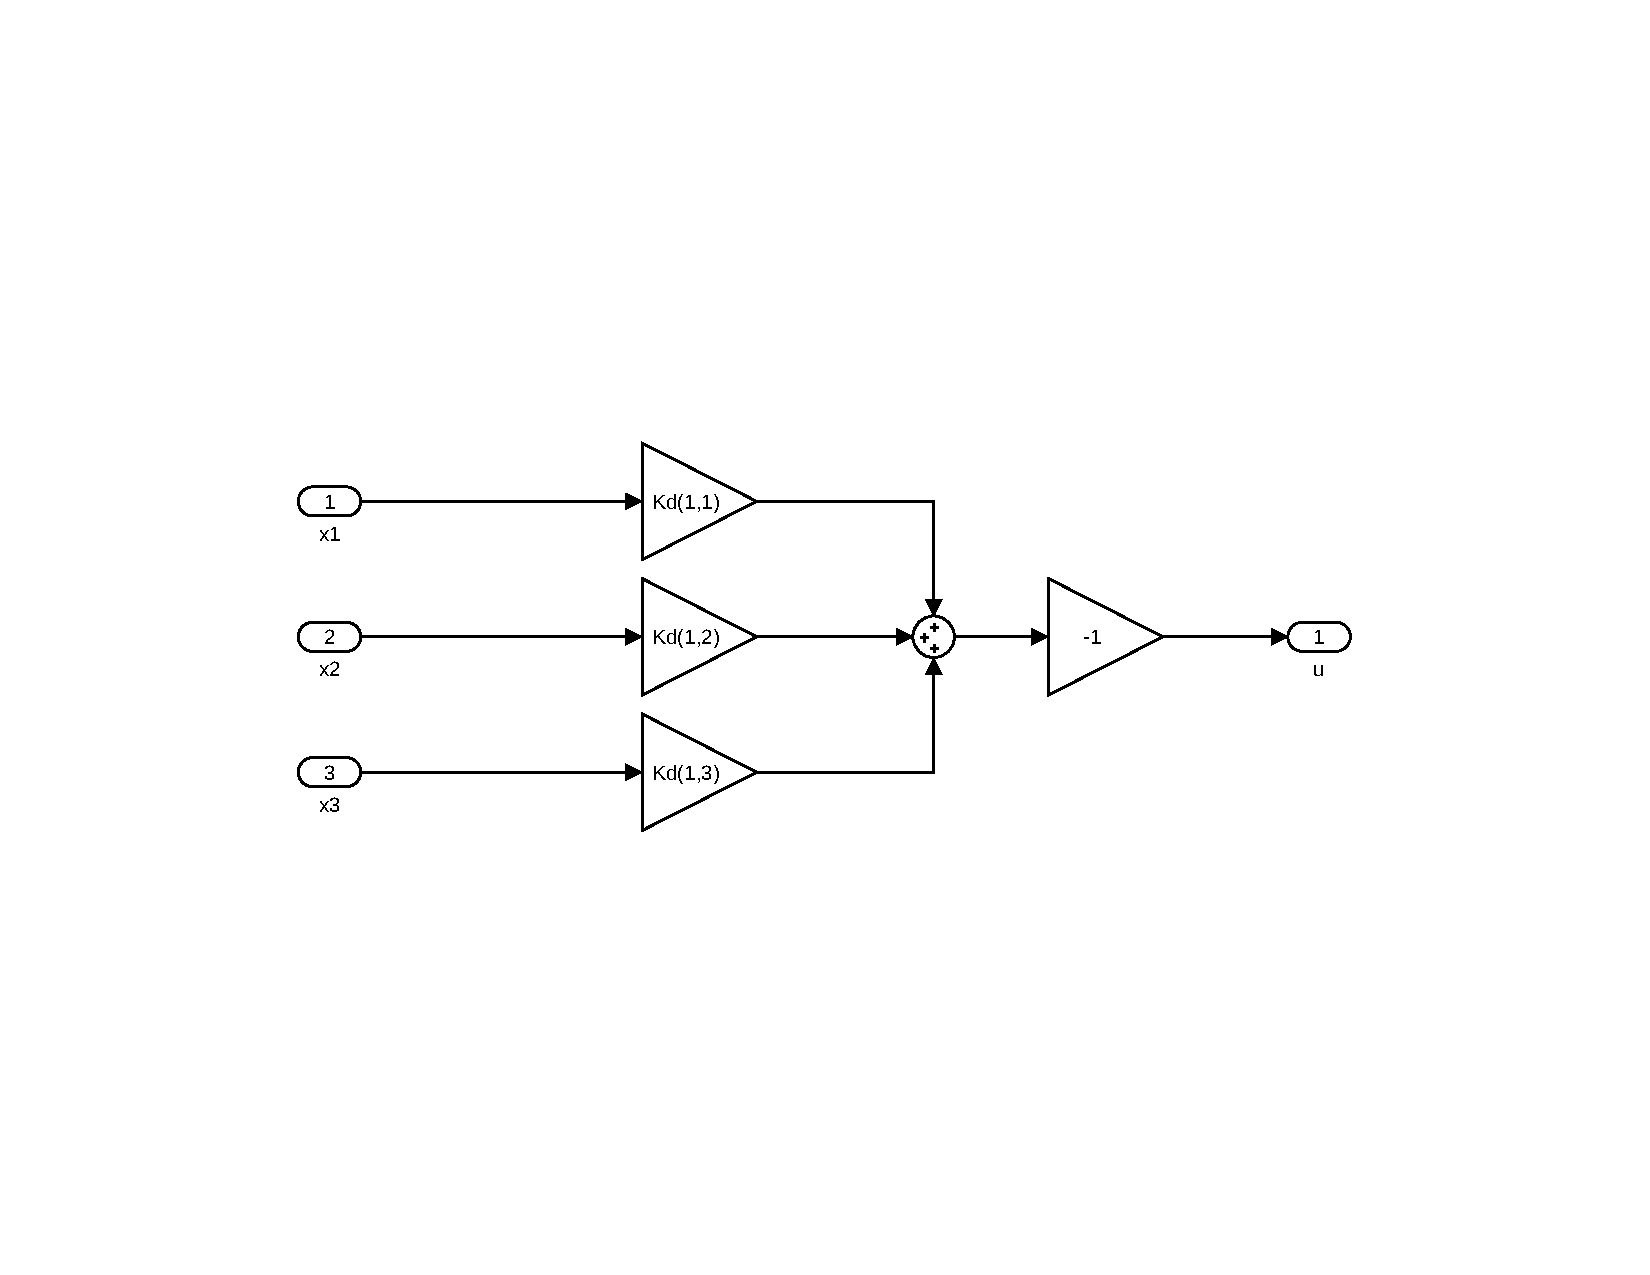
\includegraphics[width=\textwidth]{img/reg.pdf}
\caption{Struktura regulatora.}
\end{figure}

\begin{figure}[H]
\centering
 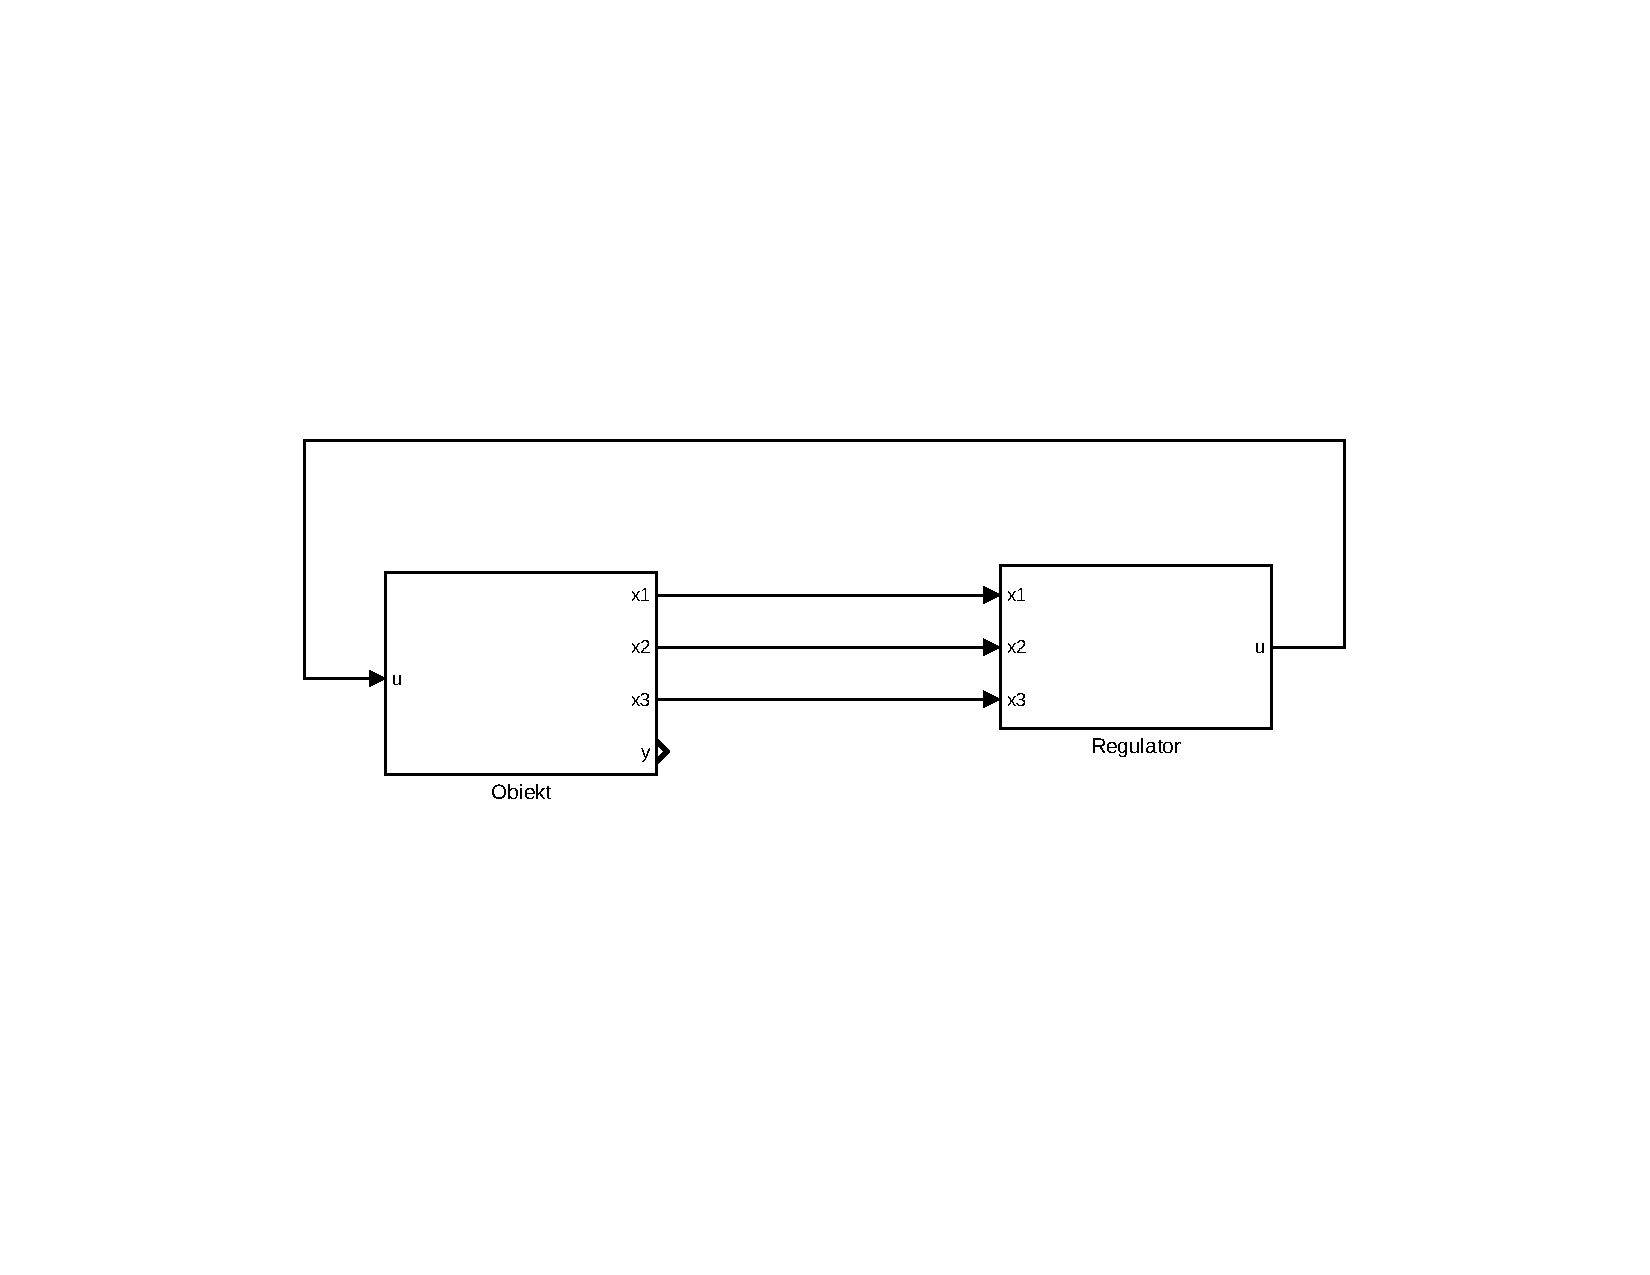
\includegraphics[width=\textwidth]{img/objreg.pdf}
\caption{Struktura układu zamkniętego.}
\end{figure}

\subsection{Trzy takie same bieguny}
Ustawiając trzy bieguny regulatora na tę samą wartość nie jesteśmy w stanie otrzymać stabilnego układu.
Układ jest najwolniej niestabilny w okolicach $z_b \approx 2,5$, co można obliczyć metodą prób i błędów.

\begin{figure}[H]
\centering
 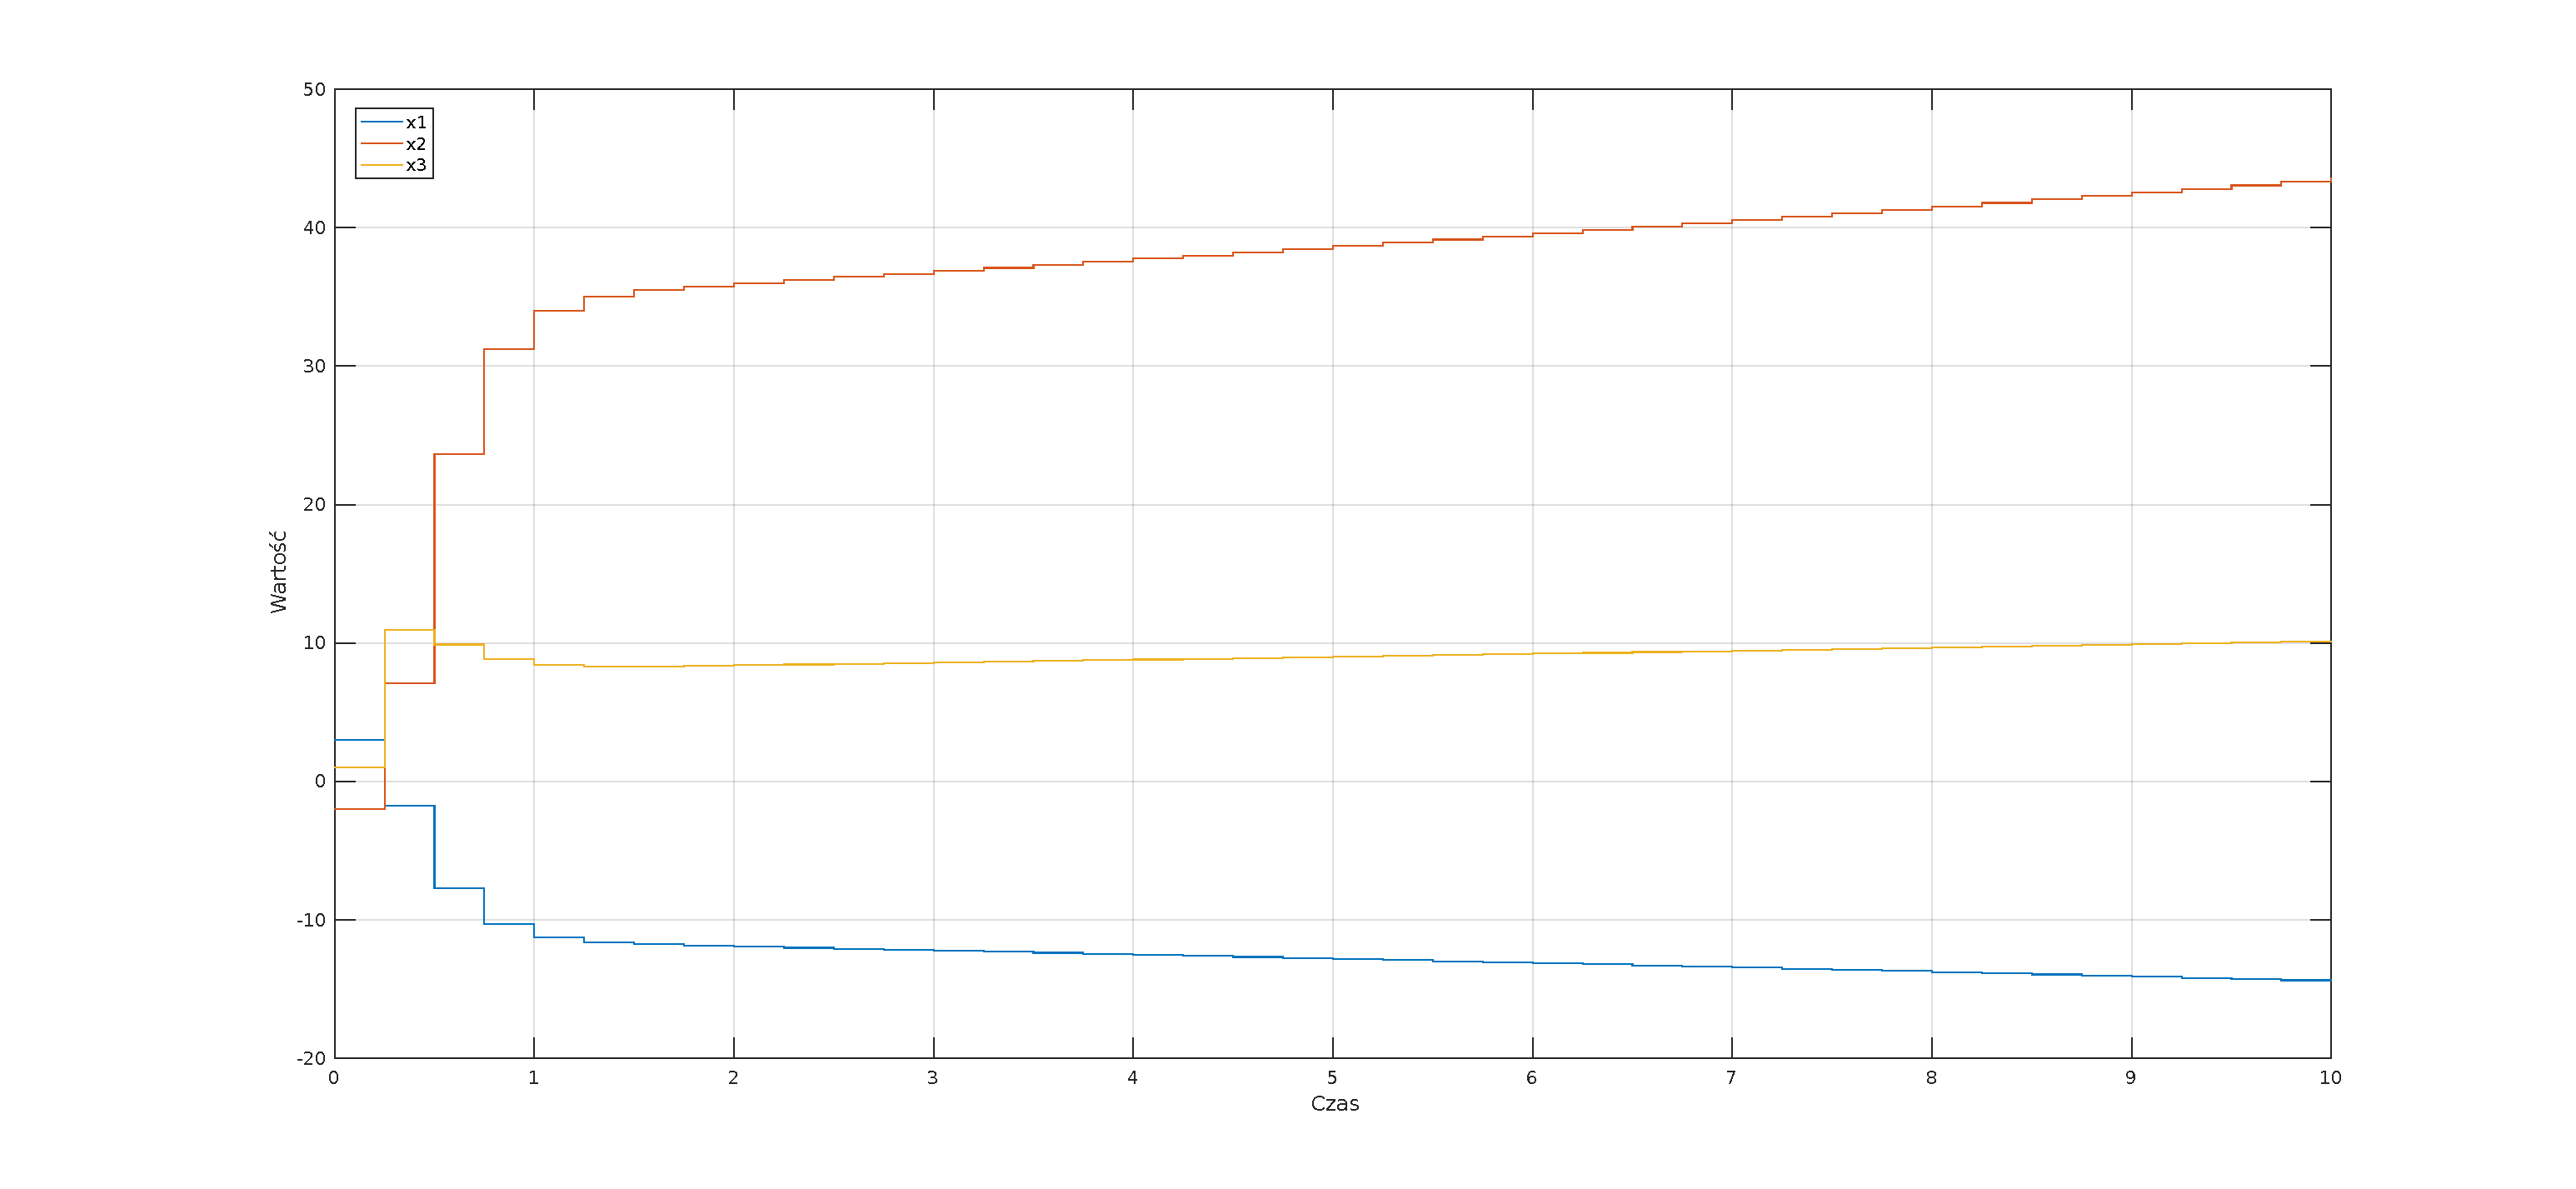
\includegraphics[width=\textwidth]{img/plot5_1.pdf}
\caption{Wartości stanu dla trzech biegunów $\approx 2,5$.}
\end{figure}

\subsection{Dwa bieguny dominujące}
Dwa bieguny powinny być szybkie, a zatem jak najbliżej środka układu współrzędnych.
Można ustalić $z_{b2} = z_{b3} = 0,1$, oraz $z_{b1} = 0,3$.
To daje nam przebieg taki, jak na wykresie.
\begin{figure}[H]
\centering
 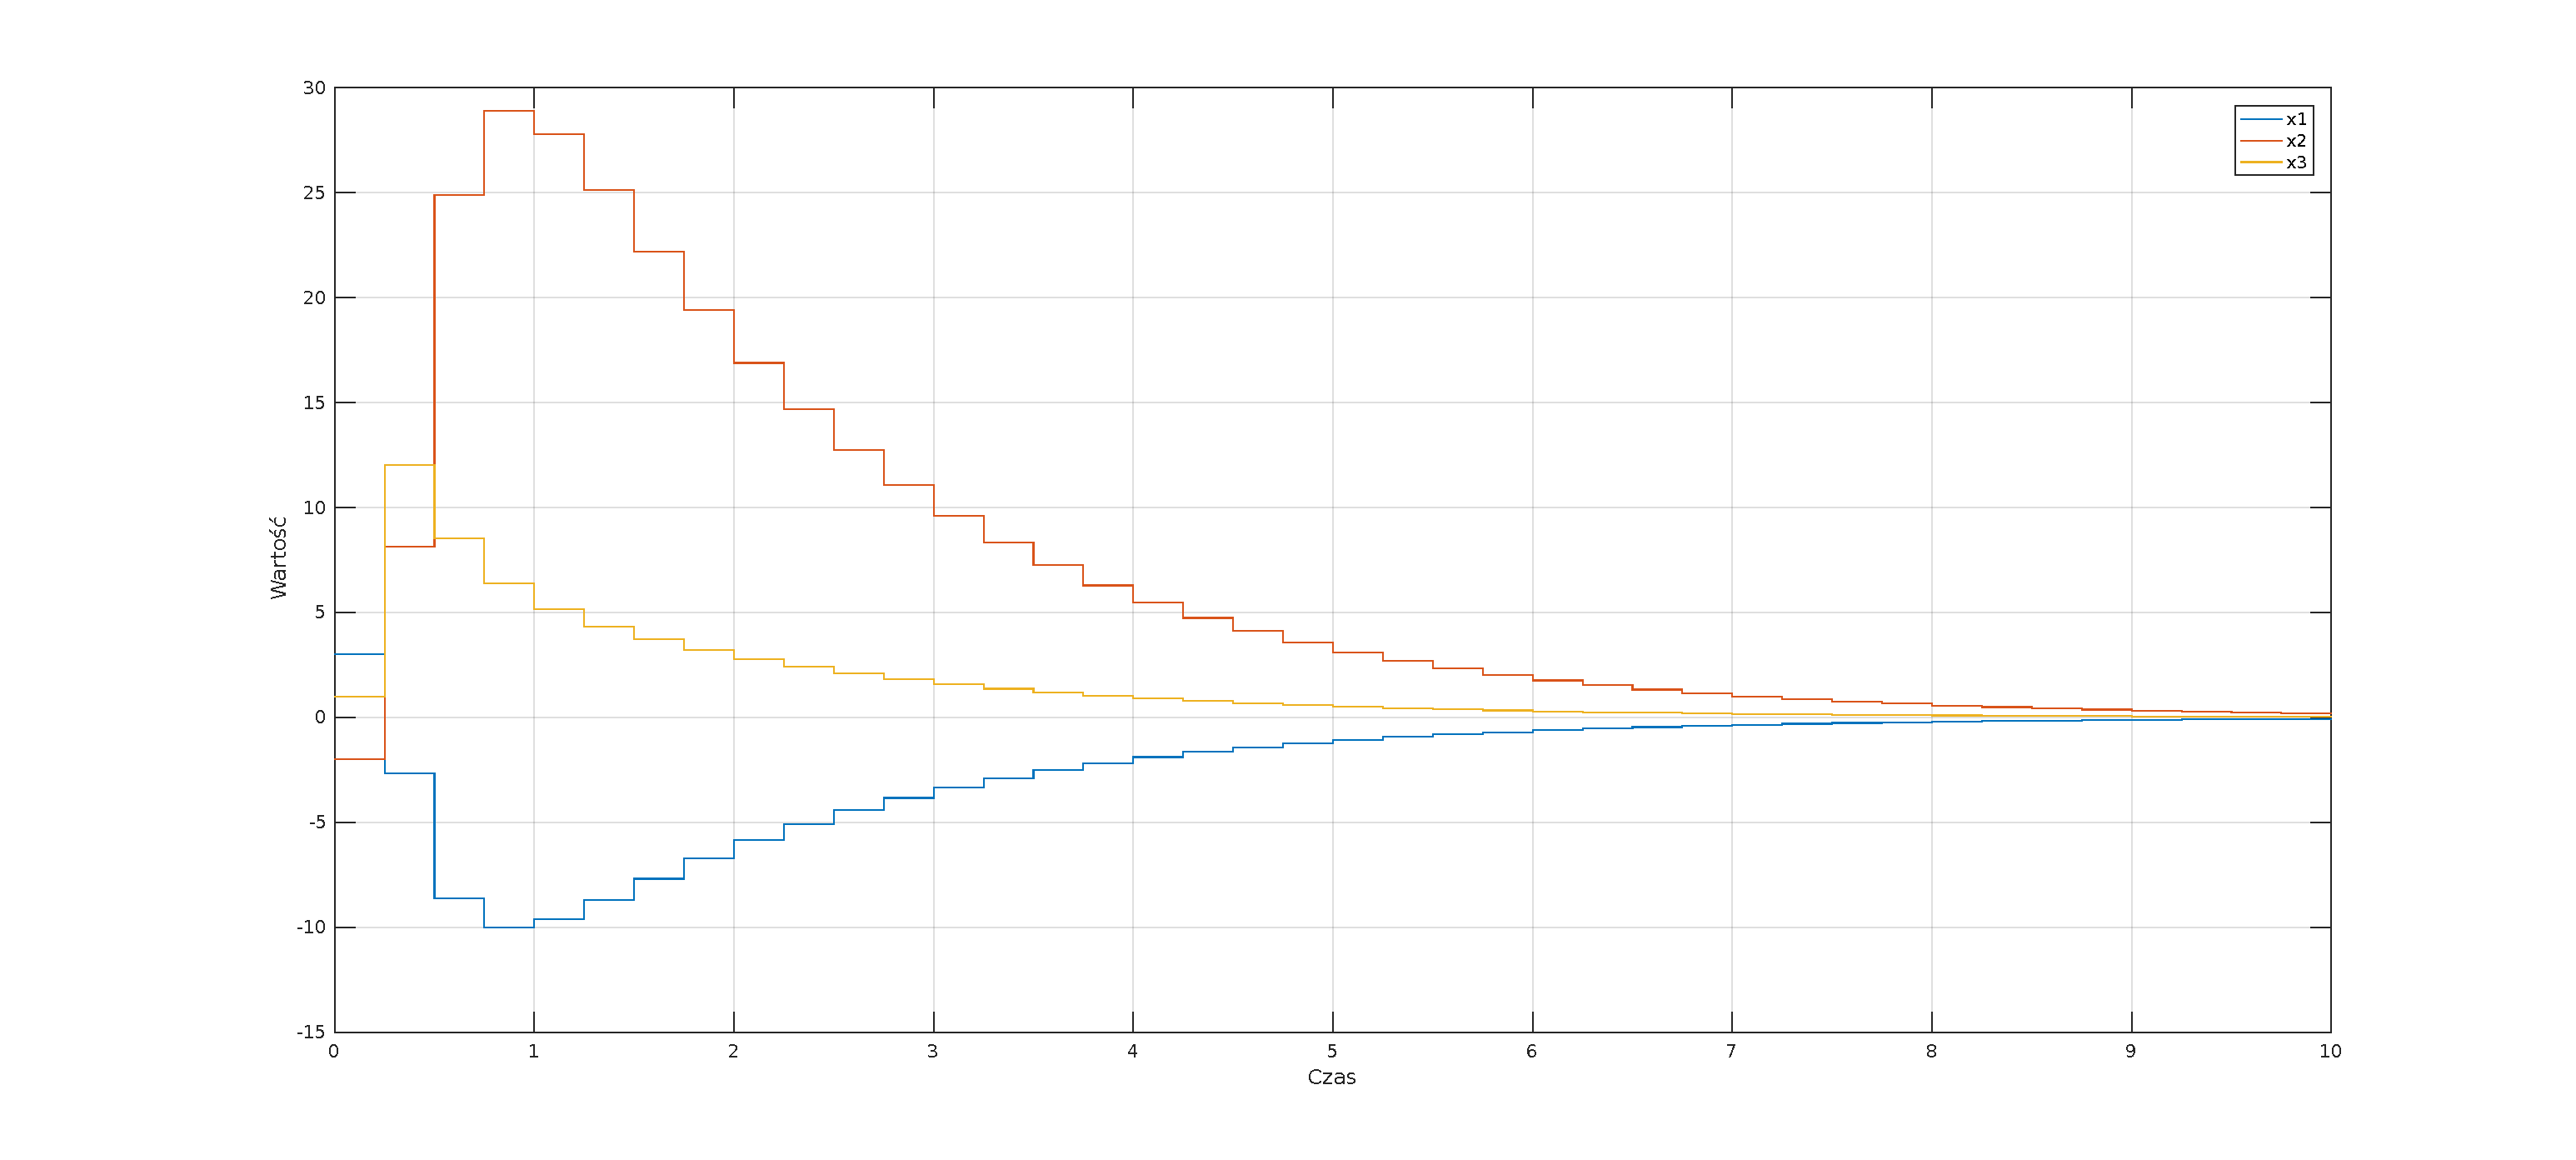
\includegraphics[width=\textwidth]{img/plot5_2.pdf}
\caption{Wartości stanu dla dwóch biegunów dominujących.}
\end{figure}
Tym razem układ jest stabilny i jego stan zbiega do 0.
Ustawienie biegunów tak, aby układ był stabilny jest bardzo trudne, wystarczy nawet niewielka zmiana w jednym z nich, aby wartości stanu uciekały w nieskończoność.

\subsection{Inne bieguny}
\begin{itemize}
\item Jeśli jeden z biegunów jest równy 0, to układ nadal jest stabilny, ale niewiele lepiej, niż w poprzednim przypadku.
\item Jeśli dwa bieguny są zerowe, to układ jest stabilny bardzo słabo. Dojście do stanu ustalonego zajmuje mu ponad 20 sekund.
\item Trzy bieguny zerowe dają układ niestabilny.

Druga wersja regulatora, z dwoma równymi biegunami, jest znacznie lepsza od trzech tych samych biegunów.

Wartość sterowania zmienia się bardzo niewiele w zależności od biegunów. 
Najlepsze przebiegi otrzymano dla trzech biegunów o malejącej szybkości $z_{b1}=0$, $z_{b2}=0,2$ i $z_{b3}=0,3$.
Taki przebieg nie dzwoni i zbiega do stanu ustalonego w rozsądnym czasie, a także nie nadwyręża układu wykonawczego.

\begin{figure}[H]
\centering
 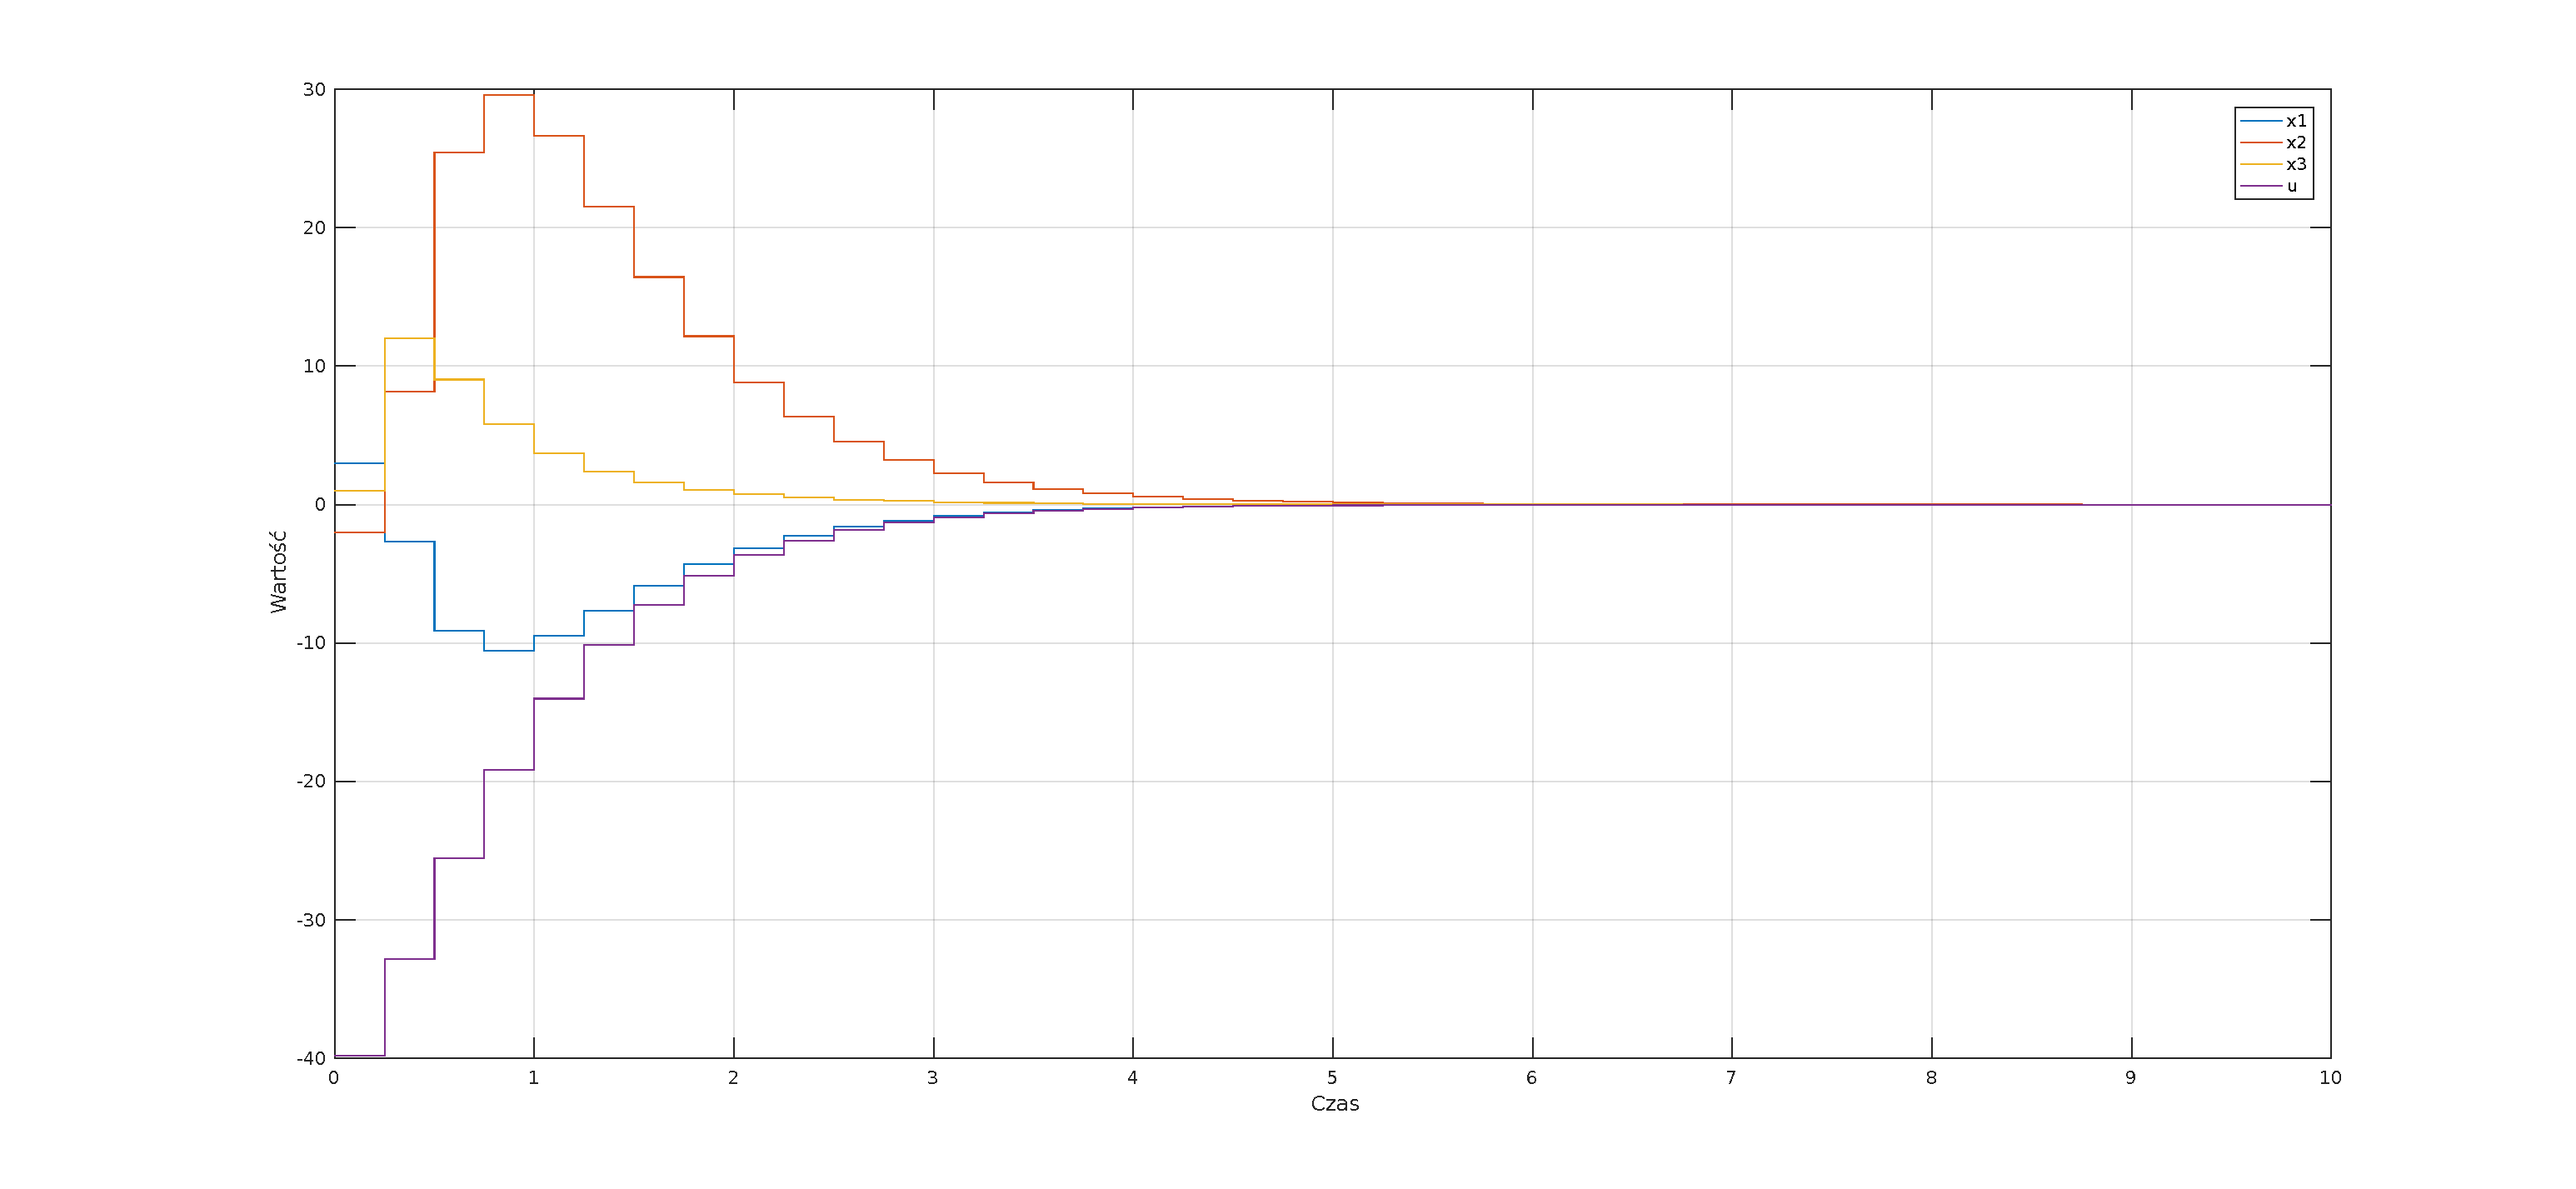
\includegraphics[width=\textwidth]{img/plot5_3.pdf}
\caption{Regulator $z_{b1}=0$, $z_{b2}=0,2$ i $z_{b3}=0,3$.}
\end{figure}

\begin{figure}[H]
\centering
 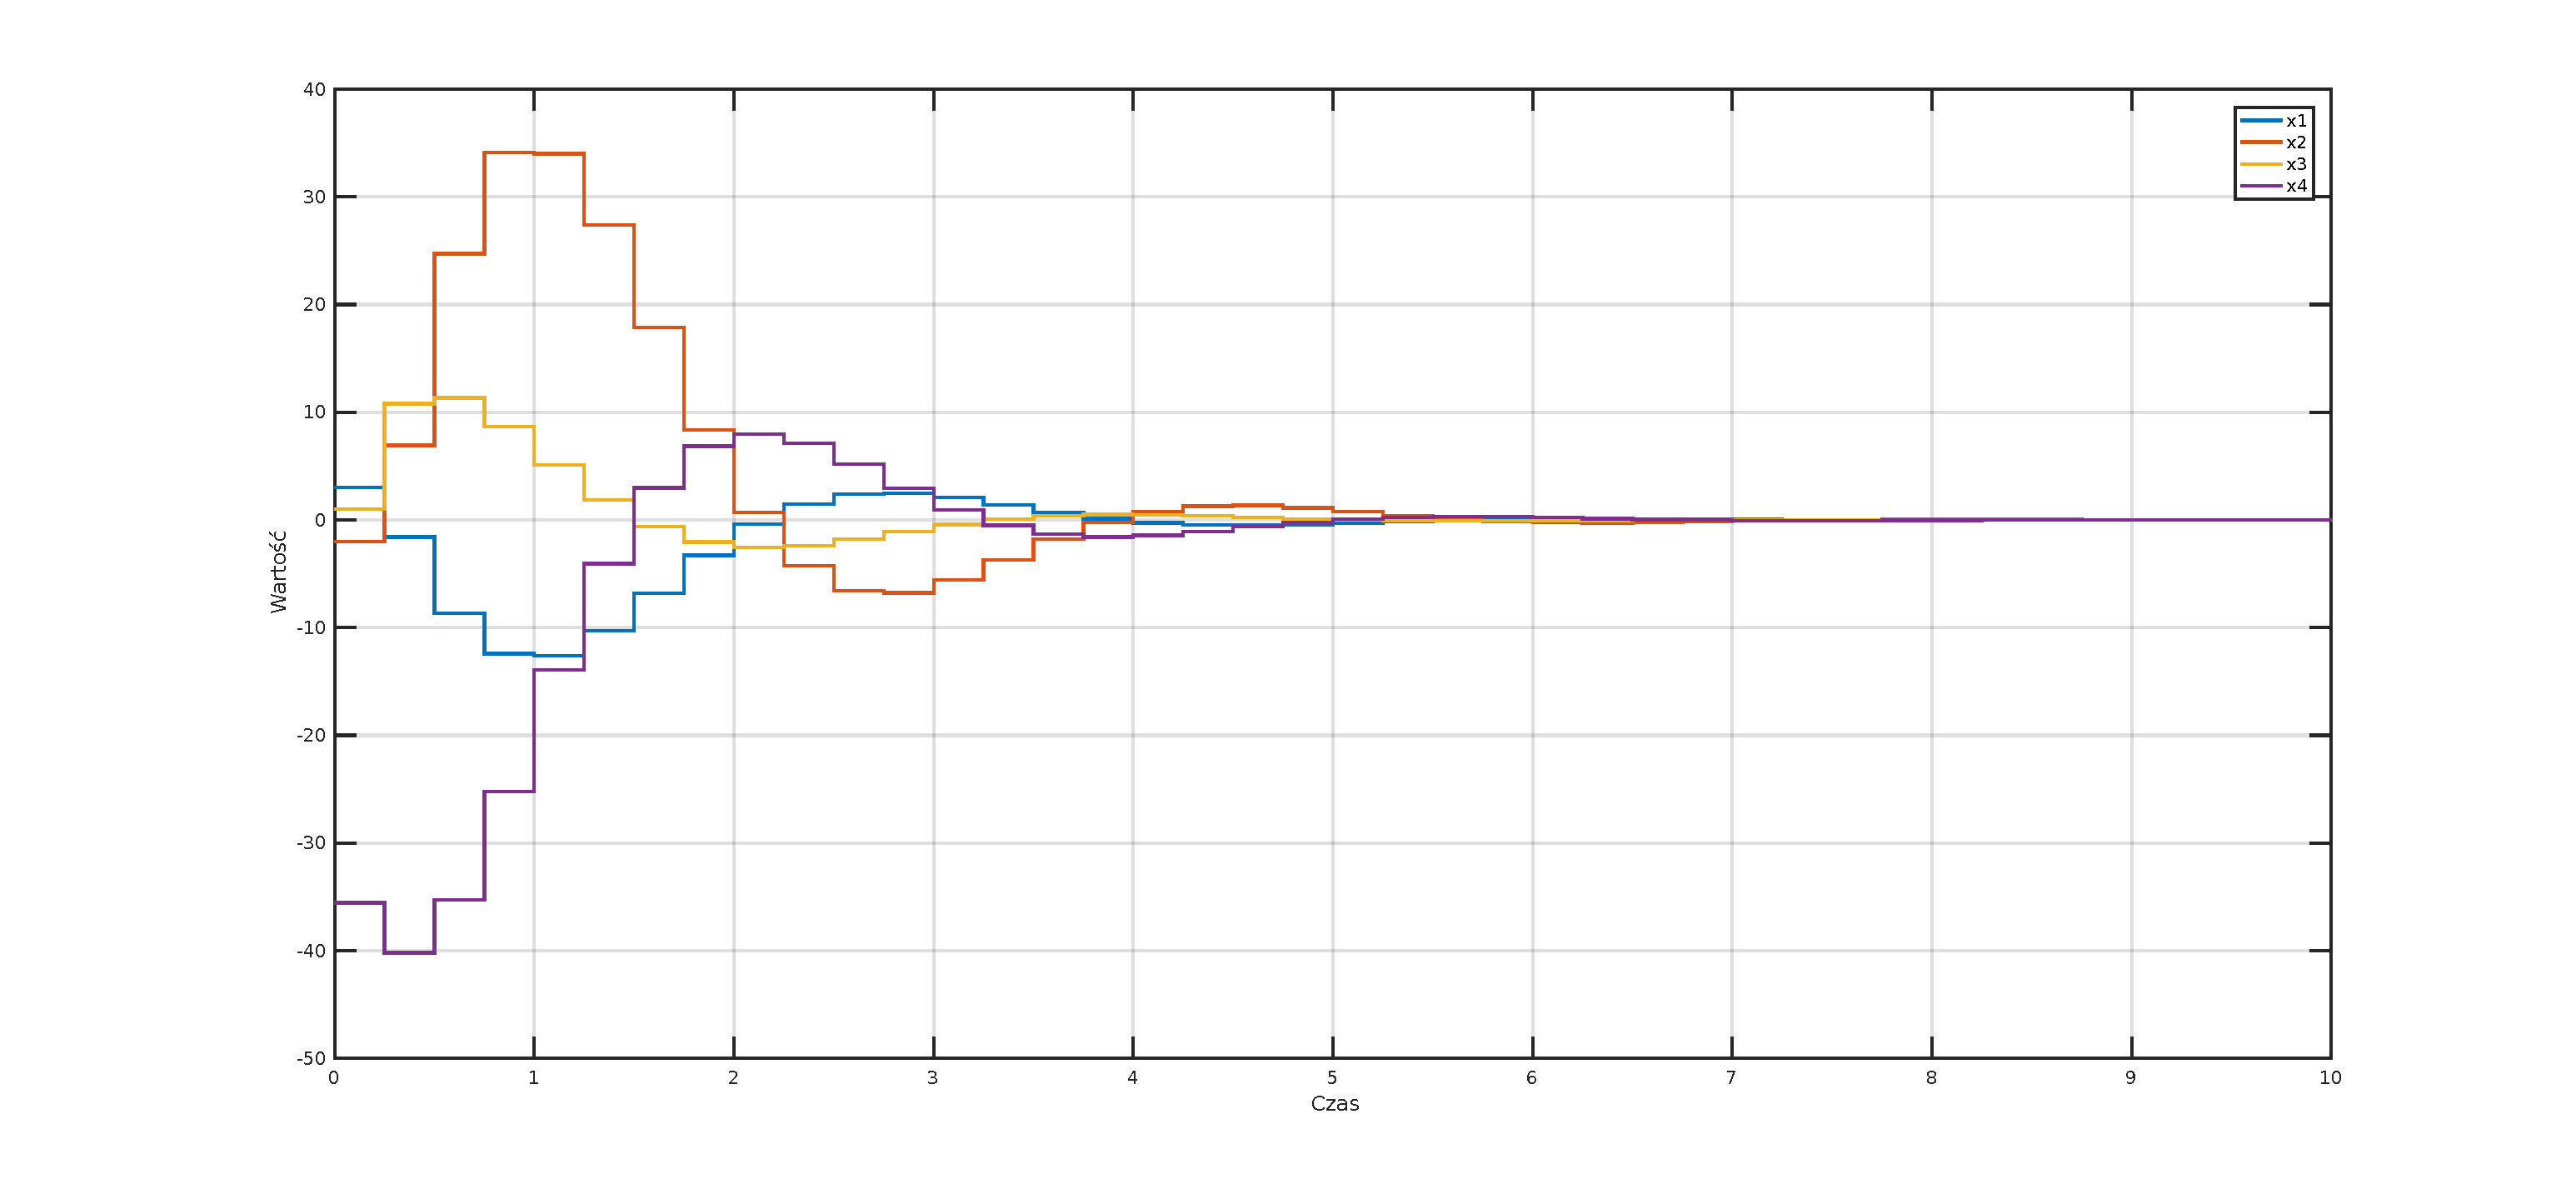
\includegraphics[width=\textwidth]{img/plot5_4.pdf}
\caption{Regulator $z_{b1}=0,2$, $z_{b2}=0,4$ i $z_{b3}=0,2$.}
\end{figure}

\begin{figure}[H]
\centering
 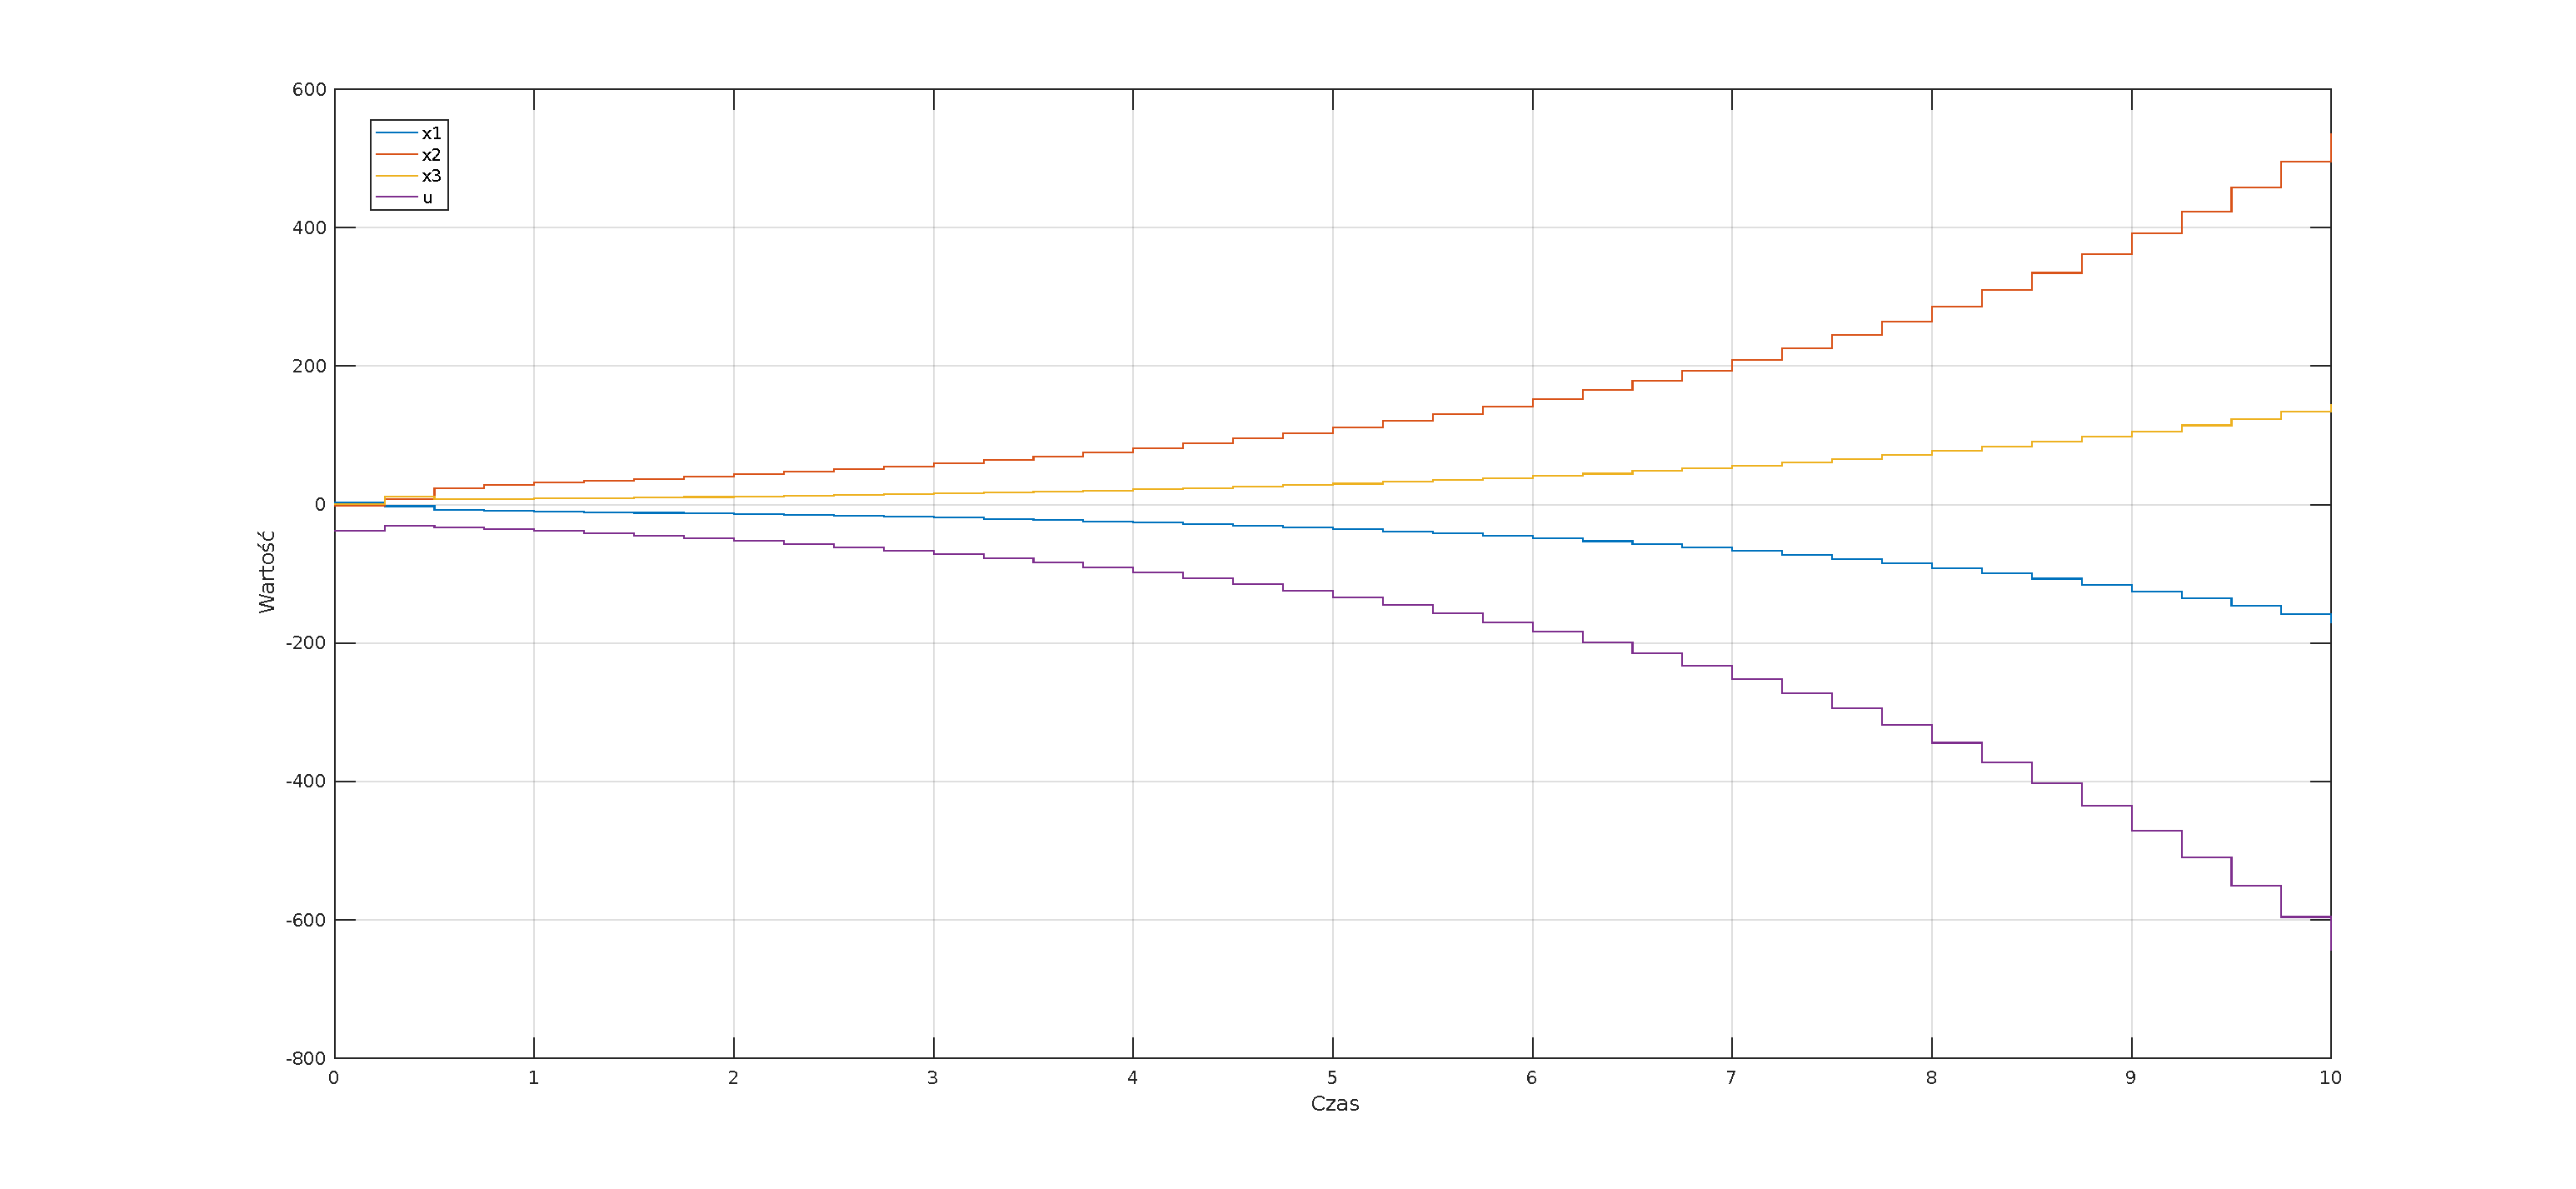
\includegraphics[width=\textwidth]{img/plot5_5.pdf}
\caption{Rozregulator $z_{b1}=0,2$, $z_{b2}=0,2$ i $z_{b3}=0,2$.}
\end{figure}

\begin{figure}[H]
\centering
 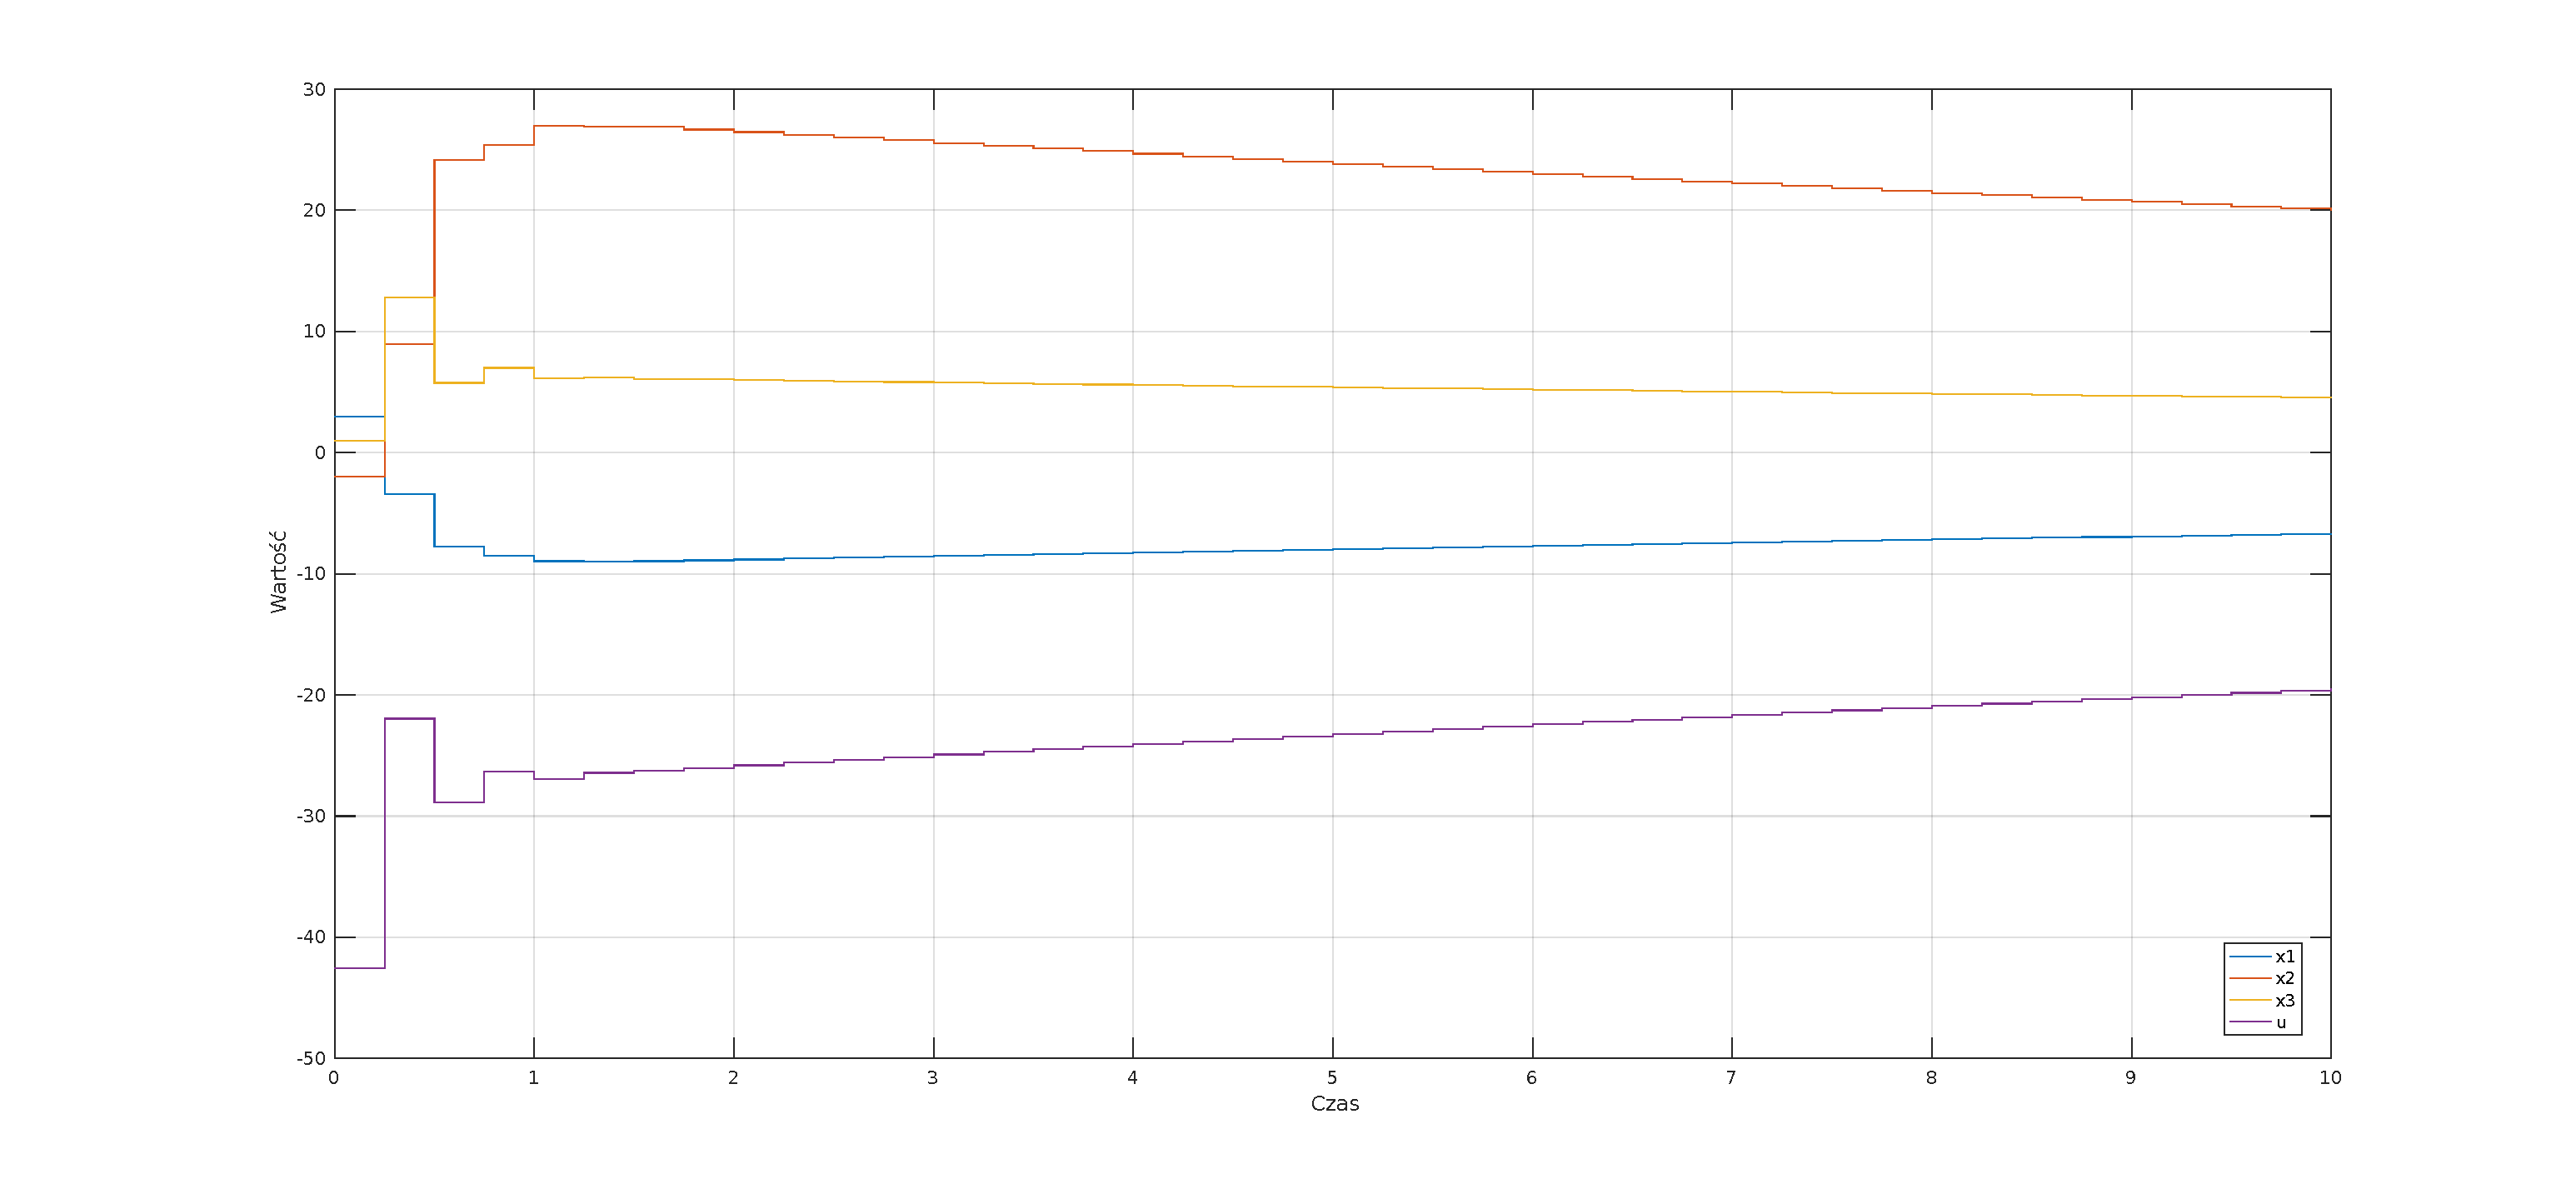
\includegraphics[width=\textwidth]{img/plot5_6.pdf}
\caption{Regulator $z_{b1}=0$, $z_{b2}=0$ i $z_{b3}=0,3$.}
\end{figure}


\end{itemize}

